% THIS TEMPLATE IS A WORK IN PROGRESS
% Adapted from an original template by faculty at Reykjavik University, Iceland

\documentclass{scrartcl}

% Adapted from an original template by Hlyni Arnórssyni, Reykjavik University, Iceland
%
% ------------------------------ SETTINGS
\usepackage{geometry}

\geometry{
	paper=a4paper, % Paper size
	top=2.5cm, % Top margin
	bottom=2.5cm, % Bottom margin
	left=2.5cm, % Left margin
	right=2.4cm, % Right margin
	headheight=0.75cm, % Header height
	footskip=1.5cm, % Space from the bottom margin to the baseline of the footer
	headsep=0.75cm, % Space from the top margin to the baseline of the header
	%showframe, % Uncomment to show how the type block is set on the page
}

\usepackage{blindtext}
%-------------------------------- Character encoding ----------------------------
\usepackage[T1]{fontenc}
\usepackage[utf8]{inputenc}

%----------------------------- Mathematics packages from AMS ---------------

\usepackage{amsmath, amsfonts, amsthm, amssymb}
\usepackage{braket, nicefrac}

% ----------- International System of Units
\usepackage{siunitx}

%------------------------------ Lists / numbers -------------------------
\usepackage{enumitem, multicol}

%------------------------------- Figure insertions --------------
\usepackage{graphicx, float}  % Use option [H] to force the placement of a figure
\usepackage{keystroke}
\usepackage{pgfplots}\usepgfplotslibrary{units}\pgfplotsset{compat=1.16}




%%%%%%%%%%%%%%%%%%%%%%%%%% Hyperlink References %%%%%%%%%%%%%%%%%%%%%%%%%%%
\usepackage{hyperref}

%--------------------% Storage Path for images %-----------------%
\graphicspath{{graphics/}{Graphics/}{./}}
\usepackage{graphicx, epsfig, booktabs}

\hypersetup{
   colorlinks   = true,                               %Colours links instead of ugly boxes
   urlcolor     = blue,                               %Colour for external hyper links
   linkcolor    = blue,                               %Colour of internal links
   citecolor    = red,                                %Colour of citations
   setpagesize  = false,
   linktocpage  = true,
}
\graphicspath{ {fig/} }



\renewenvironment{abstract}{
    \centering
    \textbf{Abstract}
    \vspace{0.5cm}
    \par\itshape
    \begin{minipage}{0.7\linewidth}}{\end{minipage}
    \noindent\ignorespaces
}
% ------------------------------------------------------------------------------------------------------------------------

\begin{document}
%Title of the report, name of coworkers and dates (of experiment and of report).
\begin{titlepage}
	\centering
	
\includegraphics[width=0.6\textwidth]{GW_logo.eps}\par
	\vspace{2cm}
	%%%% COMMENT OUT irrelevant lines below: Data Science OR Computer Science OR none
	{\scshape\LARGE Data Science Program \par}
	\vspace{1cm}
	{\scshape\Large Capstone Report - Fall 2024\par}
	%{\large \today\par}
	\vspace{1.5cm}
	%%%% PROJECT TITLE
	{\huge\bfseries Time Series Model Applications \par}
	\vspace{2cm}
	%%%% AUTHOR(S)
	{\Large\itshape Liang Gao}\par
	\vspace{1.5cm}
	Supervised by\par
	%%%% SUPERVISOR(S)
	Amir Jafari


        \newpage

	\begin{abstract}
            In this study, we compare the performance of classical time series models (AR, MA, ARMA, ARIMA) and modern deep learning techniques (LSTM, Bi-LSTM, Seq2Seq) alongside a state-of-the-art transformer model. These models have been individually studied and applied to specific problems, but the lack of a standardized benchmark for comparing their performance across diverse datasets creates a significant gap in the literature. The goal of this research is to benchmark the performance of representative time-series models across different datasets. We evaluate the models using three publicly available datasets and compare their prediction accuracy using metrics such as MSE, RMSE, and MAE. The results show that modern deep learning techniques outperform classical models, with the simplest architecture, LSTM, achieving the lowest MSE across all datasets. Although the transformer model demonstrated superior performance compared to classical models, it did not outperform the modern techniques. This suggests that for the datasets used in this study, complex transformer architectures may not be necessary to achieve optimal results. We hope our study can provide some insights into time series studies. 
	\end{abstract}
	\vfill
% Bottom of the page
\end{titlepage}
\tableofcontents
\newpage
% ------------------------------------------------------------------------------------------------------------------------
\section{Introduction}

Time series data refers to a sequence of data points collected or recorded at successive, equally spaced time intervals  \cite{adhikari2013introductory}. Time series modeling is a rapidly advancing field that has garnered significant attention from the research community in recent decades. The primary objective of time series modeling is to systematically collect and analyze historical data to develop a model that accurately represents the underlying structure of the series. This model is then used to predict future values or make forecasts based on the observed patterns in the data. 

Time series analysis is a critical area of research with applications spanning diverse fields, such as finance \cite{kim2011time}, social science \cite{box2014time}, climate science \cite{mudelsee2010climate}, energy management \cite{chou2018forecasting}, and healthcare \cite{gao2020time}. Numerous models have been developed to address specific problems in these domains, ranging from classical linear models like AR, MA, and ARIMA to advanced deep learning architectures such as LSTM and Transformers. 


The Autoregressive(AR) model has been employed to predict the instantaneous phase and frequency of neural oscillations in EEG data, demonstrating its effectiveness in real-time forward prediction for shorter intervals \cite{shakeel2020time}. Researchers such as Jafari and Jafari (2024) have utilized the Autoregressive Moving Average (ARMA) model in combination with the Levenberg-Marquardt algorithm for speech recognition applications, demonstrating its effectiveness in handling time series data in this domain \cite{jafari2024speech}. As demonstrated in the study by \cite{chimmula2020time}, the LSTM network was used to forecast the COVID-19 outbreak in Canada, predicting trends, potential stopping points, and multi-day case counts. As discussed by \cite{jin2022time}, the authors proposed a method using a Time Series Transformer (TST) to recognize fault modes in rotating machinery. They combined the TST with a time series tokenizer and demonstrated its superior fault identification capability compared to traditional CNN and RNN models.

However, there is a noticeable lack of benchmarking studies comparing these models' performances on standardized datasets. The primary objective of this study is to evaluate and compare the performance of classical time series models(linear models) \cite{box2015time}—Autoregressive(AR), Moving Average (MA), Autoregressive Moving Average (ARMA), and Autoregressive Integrated Moving Average (ARIMA)—with advanced deep learning models (non-linear models), including Long Short-Term Memory (LSTM) \cite{hochreiter1997lstm}, Bidirectional LSTM (BiLSTM) \cite{graves2005framewise}, sequence-to-sequence architectures \cite{sutskever2014seq2seq}, and the state-of-the-art Transformer model \cite{vaswani2017attention}.

In this report, we selected representative models and evaluated their performances on three publicly available datasets. [The analysis yielded insightful conclusions], which we hope will provide valuable guidance to the readers.


% ------------------------------------------------------------------------------------------------------------------------
\section{Problem Statement}
Time-series analysis is a critical field with widespread applications, and numerous models have been developed to address its challenges. The field has seen the development of numerous models, from traditional statistical approaches like Auto-Regressive (AR), Moving Average (MA), and Auto-Regressive Integrated Moving Average (ARIMA), to advanced machine learning techniques such as Long Short-Term Memory (LSTM), Sequence-to-Sequence (Seq2Seq), and the state-of-the-art Transformer model. While these models have been individually studied and applied to specific problems, the lack of a standardized benchmark for comparing their performance across diverse datasets creates a significant gap in the literature.

The goal of this research is to benchmark the performance of representative time-series models across different datasets. Each dataset was preprocessed to ensure consistency and alignment with the experimental design. These datasets were chosen to evaluate the performance of models across diverse applications, providing comprehensive insights into their strengths and limitations.

Multiple performance metrics, such as Mean Squared Error (MSE) and Root Mean Squared Error (RMSE), are employed to ensure a robust and comprehensive evaluation. These metrics provide a quantitative foundation for assessing the accuracy and reliability of each model across the datasets. Through this analysis, we aim to identify the strengths and limitations of different modeling approaches and offer insights into their applicability for diverse time series forecasting challenges.

 
% ------------------------------------------------------------------------------------------------------------------------
\section{Data}
We utilized three public and realistic datasets in this study to evaluate the performance of various time series models:
\begin{itemize}
    \item \textbf{Weather Station Beutenberg Dataset} \cite{weather2020}: This dataset contains meteorological measurements, such as temperature, humidity, and wind speed, recorded every 10 minutes, capturing fine-grained temporal variations in environmental conditions. The data was accessed from Kaggle, and the target variable is the temperature in Celsius. 
    
    \item \textbf{Power Consumption of Tetouan City} \cite{power_consumption_of_tetouan_city_849}: This dataset comprises the energy consumption data of Tetouan City, recorded at 10-minute intervals,  offering detailed observations of energy usage patterns. It offers insights into power usage patterns and facilitates the evaluation of energy forecasting models. The dataset was retrieved from the UCI Machine Learning Repository and used to forecast the power consumption in Zone 1.
    
    \item \textbf{Air Pollution Forecasting Dataset} \cite{kaggle_lstm_dataset}: This dataset includes hourly measurements of air pollutants along with meteorological features, providing insights into atmospheric quality over time. It serves as a multivariate time series dataset to assess forecasting models in pollution monitoring. The data was sourced from Kaggle, and the target variable is the pollution called PM2.5 concentration.
\end{itemize}


\section{Models}
\subsection{Classical models}
\textbf{Autoregressive (AR).}
In an Autoregressive model, we forecast the variable of interest using a linear combination of past values of the variable.
An AR process of order \( n_a \) AR(\( n_a \))  can be written as:
\[
y(t) + a_1 y(t-1) + a_2 y(t-2) + \dots + a_{n_a} y(t-{n_a}) = \epsilon(t)
\]

\textbf{Moving Average (MA).}
Rather than using past values of the forecast variable in a
regression, a moving average model uses past forecast errors. A Moving Average process of order order \( n_b \), (MA(\( n_b \))) can be represented as:
\[
y(t) = \epsilon(t) + b_1 \epsilon(t-1) + b_2 \epsilon(t-2) + \dots + b_{n_b} \epsilon(t - n_b)
\]

\textbf{Autoregressive Moving Average (ARMA).}
The Autoregressive-Moving Average model is the combination of AR and MA models, which can be represented as:
\[
y(t) + a_1 y(t-1) + a_2 y(t-2) + \dots + a_{n_a} y(t-{n_a}) = \epsilon(t) + b_1 \epsilon(t-1) + b_2 \epsilon(t-2) + \dots + b_{n_b} \epsilon(t - n_b)
\]
In comparison to pure autoregressive (AR) and moving average (MA) models, the Autoregressive Moving Average (ARMA) models offer an efficient linear approach for modeling stationary time series. This is because ARMA models can capture the underlying process of the data with fewer parameters, making them a more effective choice for such data structures. By combining both autoregressive and moving average components, ARMA models strike a balance between flexibility and simplicity in modeling time series dependencies.

\textbf{Autoregressive Integrated Moving Average (ARIMA).}
Autoregressive integrated moving average (ARIMA) model is a generalization of the autoregressive moving average model with differencing. In the general form, the ARIMA(\(n_a, d, n_b\)) model can be written as:
$$
\left(1+a_1 q^{-1}+\dots+a_{n_a} q^{-n_a}\right)\left(1-q^{-1}\right)^d y(t) = \left(1+b_1 q^{-1}+\dots+b_{n_b} q^{-n_b}\right)\epsilon(t)$$
Notation:
\begin{itemize}
    \item \( y(t) \) is the value of the time series at time \( t \),
    \item \( a_1, a_2, \dots, a_{n_a} \) are the coefficients of the AR model,
    \item \( n_a \) is the order of the autoregressive model,
    \item \( b_1, b_2, \dots, b_{n_b} \) are the coefficients of the MA model,
    \item \( n_b \) is the order of the moving average model,
    \item \( \epsilon(t) \) is a white noise (WN $\sim (0, \sigma_\epsilon^2)$),
    \item \( d \) is the number of non-seasonal order differencing.
\end{itemize}

\subsection{Modern techniques}
\textbf{Long Short-Term Memory (LSTM).}
Long Short-Term Memory (LSTM) networks, introduced by Hochreiter and Schmidhuber in 1997, are a specialized type of Recurrent Neural Network (RNN) \cite{medsker2001recurrent} designed to effectively capture long-term dependencies in sequential data \cite{hochreiter1997lstm}. Unlike traditional RNNs, which suffer from the vanishing gradient problem, LSTMs utilize a unique architecture comprising a cell state and three gates—input, forget, and output gates. These gates regulate the flow of information, enabling the network to selectively store, update, and retrieve information over extended sequences, making LSTMs particularly suitable for time series forecasting and natural language processing tasks. The architecture of the LSTM model can be represented in Figure \ref{fig:lstm}:
\begin{figure}[H]
	\begin{center}
		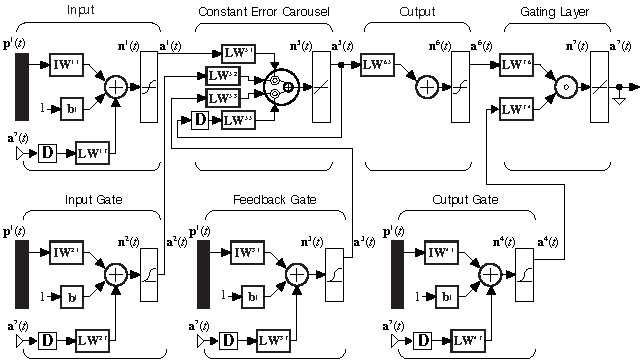
\includegraphics[scale=0.99]{Latex_report/fig/lstm.pdf}
	\end{center}
	\caption{The LSTM - Model Architecture
    \cite{nlp_lecture}}
	\label{fig:lstm}
\end{figure}

\textbf{Bidirectional Long Short-Term Memory (BiLSTM).}
Bidirectional Long Short-Term Memory (BiLSTM) networks are an advanced extension of LSTM models that process sequential data in both forward and backward directions, leveraging information from past and future contexts simultaneously. This architecture employs two separate LSTMs: one analyzing the input sequence in its original order and the other in reverse. By combining their outputs, BiLSTM networks provide a richer representation of the data, making them particularly effective for tasks like time series forecasting, natural language processing, and speech recognition \cite{graves2005framewise}.

\textbf{Sequence-to-sequence (Seq2Seq).}
Sequence-to-sequence (Seq2Seq) models are widely used for tasks requiring the transformation of input sequences into output sequences of varying lengths, such as language translation or time series forecasting. In the implemented architecture, the model follows an encoder-decoder framework enhanced by an attention mechanism:
\begin{itemize}
    \item \textbf{Encoder:} An LSTM processes the input sequence, summarizing it into a fixed-length context vector.
    \item \textbf{Attention Mechanism:} A linear layer computes attention weights, enabling the decoder to focus on relevant encoder outputs dynamically.
    \item \textbf{Decoder:} A second LSTM generates the target sequence, step-by-step, using the context vector and attention-adjusted encoder outputs.
    \item \textbf{Output Layer:} A final linear layer maps the decoder outputs to the target prediction space.
\end{itemize}
The attention mechanism addresses the limitations of fixed-length representations, improving performance on tasks involving long sequences. This architecture is inspired by the attention-based Seq2Seq models introduced by \cite{bahdanau2014neural}.

\subsection{State of Art}
\textbf{Transformer.}
The Transformer model, introduced by \cite{vaswani2017attention}, has significantly advanced deep learning with its attention mechanism and parallelized architecture. Unlike traditional recurrent models that process sequences sequentially, Transformers handle entire sequences simultaneously, making them more efficient in capturing long-term dependencies. The model consists of two main components: the encoder and the decoder. The encoder processes input sequences using self-attention and feed-forward layers, while the decoder generates outputs by attending to both the encoder's representation and previous outputs. Key features include the scaled dot-product attention, which calculates relationships between tokens using queries, keys, and values, and positional encoding, which incorporates sequence order information. Due to their capacity to model non-linear and long-range dependencies, Transformers have outperformed recurrent models in various tasks, including time series forecasting. The architecture of the Transformer model
can be represented in Figure \ref{fig:trans}:

\begin{figure}[H]
	\begin{center}
		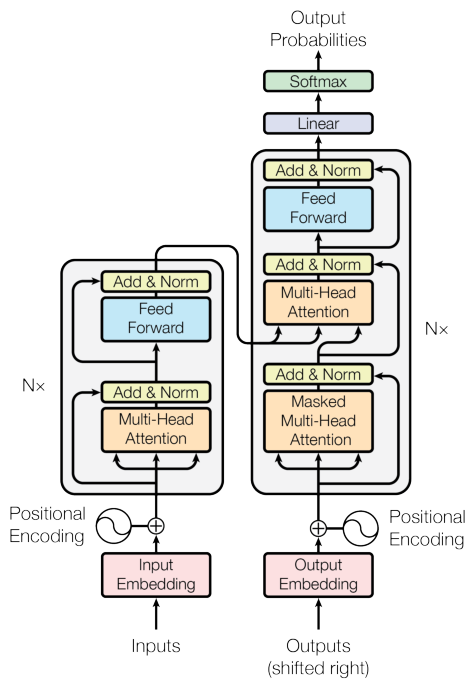
\includegraphics[scale=0.9]{Latex_report/fig/attention.pdf}
	\end{center}
	\caption{The Transformer - Model Architecture
        \cite{nlp_lecture}}
	\label{fig:trans}
\end{figure}

% ------------------------------------------------------------------------------------------------------------------------

\section{Analysis}
\label{sec:tool}
In this study, we used time series domain knowledge, including ACF/PACF plot and generalized partial autocorrelation (GPAC), to help determine the order for classical time series linear models. Besides domain knowledge, we also used a hyperparameter optimization framework - Optuna, in the experiment. These tools are introduced below. 


\textbf{ACF/PACF.}
The Autocorrelation Function (ACF) and Partial Autocorrelation Function (PACF) are fundamental tools in time series analysis \cite{box2015time, hyndman2018forecasting, chatfield2019analysis}. The ACF measures the correlation between a time series and its own lagged values. The formula for the autocorrelation at lag \(k\) is:
\[
\rho_k = \frac{\sum_{t=k+1}^{n} (X_t - \bar{X})(X_{t-k} - \bar{X})}{\sum_{t=1}^{n} (X_t - \bar{X})^2}
\]It shows how a time series is related to its previous values, with autocorrelations computed at different lag values. 
The ACF can help identify the presence of trends or seasonality, and it is useful for detecting the order of the Moving Average (MA) model. A significant autocorrelation at a specific lag indicates that past values are predictive or future values at that lag. 

The PACF is similar to the ACF but measures the correlation between a time series and its lagged values after removing the effect of intermediate lags. The formula for the Partial Autocorrelation at lag \( k \) is:
\[
\phi_{kk} = \frac{\text{Cov}(X_t, X_{t-k} \mid X_{t-1}, X_{t-2}, \dots, X_{t-k+1})}{\sqrt{\text{Var}(X_t) \cdot \text{Var}(X_{t-k})}}
\]The PACF shows the direct correlation between a value and its lagged version without the interference of other intervening time lags. The PACF is particularly useful in identifying the order of the Autoregressive (AR) model. 

In time series modeling, the comparison of ACF (Autocorrelation Function) and PACF (Partial Autocorrelation Function) plots helps determine the underlying pattern of the data, aiding in the selection of an appropriate model. When the ACF plot gradually tails off while the PACF plot cuts off after a certain lag, it suggests an Autoregressive (AR) model. On the other hand, if the ACF plot cuts off and the PACF plot tails off, it indicates a Moving Average (MA) model. This behavior reflects the distinct structures of AR and MA processes, where AR models depend on past values, while MA models are based on past error terms. 


\textbf{GPAC.}
The Generalized Partial Autocorrelation (GPAC) is a tool used in time series analysis, particularly in the context of Auto-Regressive Moving-Average (ARMA) modeling. It is used to estimate the order of the ARMA model when the auto-regressive (AR) and moving-average (MA) orders (\( n_a \) and \( n_b \), respectively) are not known prior.

The formula to calculate the generalized partial autocorrelation can be written as:

\[
\phi_{kk}^j = 
\frac{
\begin{vmatrix}
\hat{R}_y(j) & \hat{R}_y(j-1) & \cdots & \hat{R}_y(j+1) \\
\hat{R}_y(j+1) & \hat{R}_y(j) & \cdots & \hat{R}_y(j+2) \\
\vdots & \vdots & \ddots & \vdots \\
\hat{R}_y(j+k-1) & \hat{R}_y(j+k-2) & \cdots & \hat{R}_y(j+k)
\end{vmatrix}
}{
\begin{vmatrix}
\hat{R}_y(j) & \hat{R}_y(j-1) & \cdots & \hat{R}_y(j-k+1) \\
\hat{R}_y(j+1) & \hat{R}_y(j) & \cdots & \hat{R}_y(j-k+2) \\
\vdots & \vdots & \ddots & \vdots \\
\hat{R}_y(j+k-1) & \hat{R}_y(j+k-2) & \cdots & \hat{R}_y(j)
\end{vmatrix}
}
\]

The GPAC array table  provides a visual representation of the GPAC coefficients:
$$\text{GPAC array table}$$

$$\begin{array}{c|ccccc}
j & k=1 & k=2 & \dots & k=n_a \\
\hline
0 & \phi_{11} & \phi_{22} & \dots & \\
1 & \phi_{11} & \phi_{22} & \dots & \\
\vdots & \vdots & \vdots & \ddots & \\
n_b & & & & \phi_{n_a n_a}
\end{array}$$ The rows represent the lag $j$, starting from 0 up to $n_b$. Second, the columns represent the lag $k$, starting from 1 up to $n_a$. The cells contain the GPAC coefficients $\phi_{kk}$.

The first row of the GPAC array table, in fact, the partial autocorrelation (PAC) function, which is used to estimate the order of the auto-regressive (AR) component of the ARMA model when \( n_b \) = 0.

The pattern observed in the GPAC table, where a column has constant values and a row consists entirely of zeros, identifies the orders of \( n_a \) for the AR component and \( n_b \) for the MA component. Specifically, the row number represents the MA order, while the column number indicates the AR order. This structure provides a systematic approach to determining the appropriate parameters for ARMA modeling.

\textbf{Optuna.}
In addition to using the time series domain knowledge (ACF/PACF plots and GPAC table), we also use Optuna to determine the order of classical linear time series models. Optuna is an open-source hyperparameter optimization framework designed for efficiency and flexibility in machine learning and deep learning workflows \cite{akiba2019optuna}. It employs an automated search algorithm, primarily based on Bayesian optimization, to find optimal hyperparameter configurations. Optuna uses a trial-and-error approach within a user-defined search space and supports pruning techniques to eliminate unpromising trials early, significantly reducing computation time. Its integration with major machine learning libraries and visualization tools makes it a versatile choice for both researchers and practitioners.  


% ------------------------------------------------------------------------------------------------------------------------
\section{Experimentation setting}
Our experiments were conducted using AWS cloud computing resources tailored to the computational needs of the models. Classical time series models—AR, MA, ARMA, and ARIMA—were executed on AWS CPU instances, as these models are computationally lightweight. On the other hand, the deep learning models, including LSTM, BiLSTM, Seq2Seq, and Transformer, required substantial computational power and were, therefore, trained on AWS GPU instances to ensure efficiency and faster convergence. 

To ensure a fair comparison between different models, we standardized the hyperparameter settings across the modern techniques (LSTM, BiLSTM, Seq2Seq) and the state-of-the-art Transformer model. The following hyperparameters in Table \ref{tab:hyperparams} were kept consistent across all models:

\begin{table}[h]
\centering
\begin{tabular}{lc}
\hline
\textbf{Hyperparameter}         & \textbf{Value} \\ \hline
Sequence Length                 & 6              \\ 
Batch Size                      & 128            \\ 
Optimizer                       & Adam           \\ 
Training Epochs       & 100            \\ 
Learning Rate                   & 0.001          \\ \hline
\end{tabular}
\caption{Hyperparameter Settings for Model Comparison}
\label{tab:hyperparams}
\end{table}

Additionally, for the modern techniques (LSTM, BiLSTM, Seq2Seq), we used the same number of layers, which is 1, and the same number of hidden sizes, which is 2. This uniformity in hyperparameters was designed to ensure the comparability of results across different models and to isolate the impact of model architecture on performance.

For the Optuna setting, we set the max order for the AR process to 20, the MA process to 10, and the number of trials to 30. The datasets were divided into training and validation subsets, with 80\% of the data used for training and 20\% for validation. This split ensured sufficient data for model learning while reserving a robust validation set to assess performance. To ensure the comparability of different models across various datasets, we normalized the data before calculating the MSE, RMSE, and MAE using the min-max normalization equation \ref{nomalize}.
\begin{equation}
\text{X}_{\text{normalized}} = \frac{\text{X} - \text{X}_{\min}}{\text{X}_{\max} - \text{X}_{\min}}
\label{nomalize}
\end{equation}


\section{Discussion and Conclusion}
In this study, we analyzed the characteristics of three datasets and systematically investigated the performance of various models on these datasets. In the following sections, we provide a comprehensive discussion of our findings and insights.

\subsection{Exploratory Data Analysis}
In the temperature dataset, I used the drift method to fill the 9 missing values. There are no missing values in the other two datasets. We performed Exploratory Data Analysis (EDA) to examine the characteristics of the datasets and identify underlying patterns. Various visualizations were created, including sequence plots to observe trends over time and rolling mean and variance plots to assess stationarity; we also generated autocorrelation function (ACF) and partial autocorrelation function (PACF) plots to identify potential model orders and conducted time series decomposition to analyze seasonal, trend, and residual components. The details of ACF and PACF are presented in Section \ref{sec: tool}. These analyses provided essential insights for model development. Figure \ref{fig:eda_plot} presents all the visualizations generated for our selected datasets.
\begin{figure}[H]
	\begin{center}
		\includegraphics[scale=0.90]{Latex_report/fig/pdfresizer.com-pdf-crop.pdf}
	\end{center}
	\caption{EDA plots}
	\label{fig:eda_plot}
\end{figure}

\begin{table}[ht]
\centering
\caption{Strength of Trend and Seasonality for Each Dataset}
\label{tab:trend_seasonality}
\scalebox{0.9}{ % Adjust the scale factor as needed
\begin{tabular}{lcc}
\hline
\textbf{}        & \textbf{Strength of Trend (\%)} & \textbf{Strength of Seasonality (\%)} \\ \hline
Weather                 & 94.33                          & 74.79                                 \\ 
Air Pollution           & 86.01                          & 40.67                                 \\ 
Power Consumption       & 92.41                          & 98.64                                 \\ \hline
\end{tabular}
}
\end{table}

All three datasets exhibit stationarity, as indicated by the constancy of rolling mean and variance after considering all samples. The ACF tail-off and PACF cut-off in all three datasets indicate clear AR patterns. Using time series decomposition, we calculated the strengths of trend and seasonality. Table~\ref{tab:trend_seasonality} summarizes the strength of trend and seasonality for the three datasets analyzed in this study. For the Weather dataset, the trend strength is remarkably high at 94.33\%, while the seasonality is moderate at 74.79\%. The Air Pollution dataset shows a significant trend strength of 86.01\% but relatively weak seasonality at 40.67\%. Finally, the Power Consumption dataset exhibits both a strong trend (92.41\%) and an exceptionally high seasonality (98.64\%). These metrics underline the varying characteristics of each dataset, guiding appropriate model selection.



\subsection{Classical models}
We implemented four classical linear time series models: AR, MA, ARMA, and ARIMA, each representing different approaches to modeling the temporal dependencies in time series data. Determining the appropriate model order \(n_a\) for the Autoregressive (AR) component and \(n_b\) for the moving average (MA) component is a critical step in the modeling process. To achieve this, we relied on two fundamental tools from the time series analysis domain. First, the ACF (Autocorrelation Function) and PACF (Partial Autocorrelation Function) plots were used to examine the relationships between lags. These plots provide visual cues to identify the potential order of the AR and MA components by observing the cutoff or tail-off patterns in the respective plots. Second, the GPAC (Generalized Partial Autocorrelation) table in Table \ref{fig:gpac} was utilized to systematically assess the lag patterns, offering a structured approach to infer the AR and MA orders from the data.

For the AR model, we determined the order based on the ACF and PACF plots shown in Figure \ref{fig:eda_plot}. The ACF tails off, while the PACF cuts off after a specific lag, which we used as the order for the AR model. For the MA model, since none of the ACF or PACF plots exhibited a clear MA pattern, we set the maximum MA order to 10 and employed Optuna to identify the optimal order. The GPAC table in Figure \ref{fig:gpac1} was used to determine the order for the ARMA model. Specifically, the column with constant values indicates the order for the AR component, while the row with all values equal to zero indicates the MA component order. The ARIMA model is designed to handle non-stationary datasets, where the number of non-seasonal differencing steps required to make the data stationary defines the integrated component of the model. Since our datasets are already stationary, applying differencing is not strictly necessary. However, from a technical perspective, the ARIMA model remains valid. To ensure consistency and facilitate a fair comparison with other models, we applied first-order differencing to the data and then analyzed the differenced data using the GPAC method. The table in \ref{fig:gpac2} shows the GPAC tables for our differences data. This approach allowed us to identify patterns and determine the appropriate AR and MA orders, enabling us to implement the ARIMA model effectively for comparative purposes.

\begin{figure}[H]
	\begin{center}
		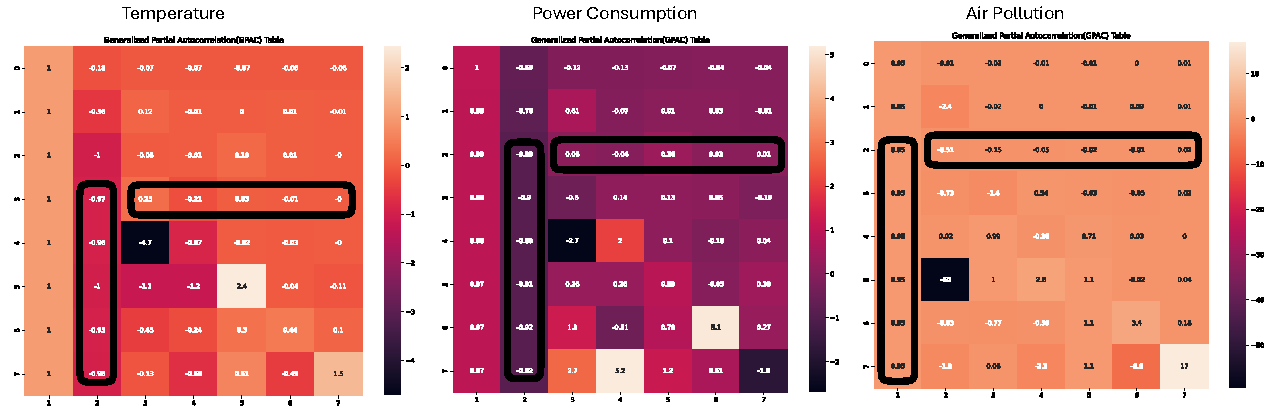
\includegraphics[scale=0.7]{Latex_report/fig/gpac1.pdf}
	\end{center}
	\caption{GPAC for Raw Data}
	\label{fig:gpac1}
\end{figure}

\begin{figure}[H]
	\begin{center}
		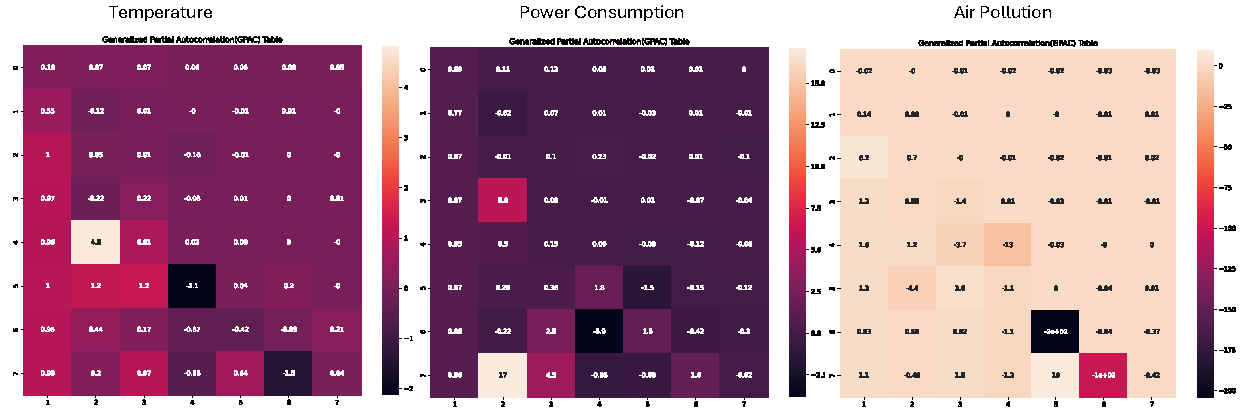
\includegraphics[scale=0.7]{Latex_report/fig/gpac2.pdf}
	\end{center}
	\caption{GPAC for Differenced  Data}
	\label{fig:gpac2}
\end{figure}


While traditional approaches like domain expertise and manual interpretation of plots were essential, we also employed Optuna, an advanced machine learning optimization algorithm, to automate and enhance the hyperparameter tuning process. By leveraging Optuna's efficient search strategies, we ensured that the selected hyper-parameters minimized errors and improved model performance, complementing the traditional methods with modern computational techniques. For the AR component, we set the max potential order to 20 and 10 for the MA component since there is no MA pattern from ACF and PACF plots. The number of trials for the AR model is 20, MA is 10, and 30 for the ARMA and ARIMA models. 

Table \ref{tab:optuna} presents the model orders determined using time series domain knowledge and those obtained via Optuna, along with their respective MSE values. As shown in the table, the differences in MSE between the two methods are minor. This suggests that while domain knowledge can be a valuable tool for determining the appropriate model order, using Optuna is a viable alternative, especially in scenarios where domain knowledge is insufficient or when it is challenging to determine an appropriate order based on the available information. Employing Optuna in such cases provides a systematic and automated approach to optimize model performance without heavily relying on prior knowledge. 


\begin{table}[h!]
\centering
\begin{tabular}{@{}lcccc@{}}
\toprule
\textbf{}               & \textbf{Domain Order}           & \textbf{MSE}     & \textbf{Optuna Order} & \textbf{MSE}     \\ \midrule
\textbf{AR}             &                                 &                  &                       &                  \\
Temperature             & (2)                             & 0.038986         & (4)                   & 0.038950         \\
Power Consumption       & (2)                             & 0.059108         & (10)                  & 0.059213         \\
Air Pollution           & (1)                             & 0.019484         & (5)                   & 0.019482         \\ \midrule
\textbf{MA}               &                                 &                  &                       &                  \\
Temperature             & --                              & --               & (10)                  & 0.038870         \\
Power Consumption       & --                              & --               & (10)                  & 0.059218         \\
Air Pollution           & --                              & --               & (10)                  & 0.019472         \\ \midrule
\textbf{ARMA}             &                                 &                  &                       &                  \\
Temperature             & (2,3)                           & 0.038971         & (8,2)                 & 0.038892         \\
Power Consumption       & (2,2)                           & 0.059206         & (4,5)                 & 0.059281         \\
Air Pollution           & (1,2)                           & 0.019483         & (2,6)                 & 0.019458         \\ \midrule
\textbf{ARIMA}            &                                 &                  &                       &                  \\
Temperature             & (1,1,1)                         & 0.049111         & (7,1,6)               & 0.044493         \\
Power Consumption       & (1,1,2)                         & 0.055292         & (11,1,6)              & 0.055068         \\
Air Pollution           & (4,1,5)                         & 0.019482         & (13,1,10)             & 0.019479         \\ \bottomrule
\end{tabular}
\caption{MSE Comparison between Domain Knowledge and Optuna. Both prediction and ground truth are normalized using the equation in \ref{nomalize}.}
\label{tab:optuna}
\end{table}

We selected the order with the lower MSE from those determined using domain knowledge and Optuna as the final order for each model. To evaluate the performance of the four classical models, we computed MSE, RMSE, and MAE, with the results presented in Table \ref{tab:classical_metric}. The comparison between predicted and actual values is visualized in Figure \ref{fig: classical}. It is evident that the performance of the classical models is not very satisfactory, which is reasonable given that these models were designed using the simplest possible approaches based solely on the available information, serving primarily as baseline references.
\begin{table}[h!]
\centering
\begin{tabular}{@{}lccc@{}}
\toprule
\textbf{}               & \textbf{MSE} & \textbf{RMSE} & \textbf{MAE} \\ \midrule
\textbf{AR}             &              &               &              \\
Temperature             & 0.038950     & 0.197359      & 0.161282     \\
Power consumption       & 0.059108     & 0.243121      & 0.204268     \\
Air pollution           & 0.019482     & 0.139578      & 0.101504     \\ \midrule
\textbf{MA}             &              &               &              \\
Temperature             & 0.038870     & 0.197156      & 0.160967    \\
Power consumption       & 0.059218     & 0.243347      & 0.204480     \\
Air pollution           & 0.019472     & 0.139542      & 0.101515     \\ \midrule
\textbf{ARMA}           &              &               &              \\
Temperature             & 0.038892     & 0.197210      & 0.161051     \\
Power consumption       & 0.059206     & 0.243322      & 0.204456     \\
Air pollution           & 0.019458     & 0.139493      & 0.101845      \\ \midrule
\textbf{ARIMA}          &              &               &              \\
Temperature             & 0.044493     & 0.210933      & 0.178464     \\
Power consumption       & 0.055068     & 0.234666      & 0.193346     \\
Air pollution           & 0.019479     & 0.139569      & 0.101566       \\ \bottomrule
\end{tabular}
\caption{Performance metrics for Classical Models. Both prediction and ground truth are normalized using the equation in \ref{nomalize}.}
\label{tab:classical_metric}
\end{table}


\begin{figure}[]
	\begin{center}
		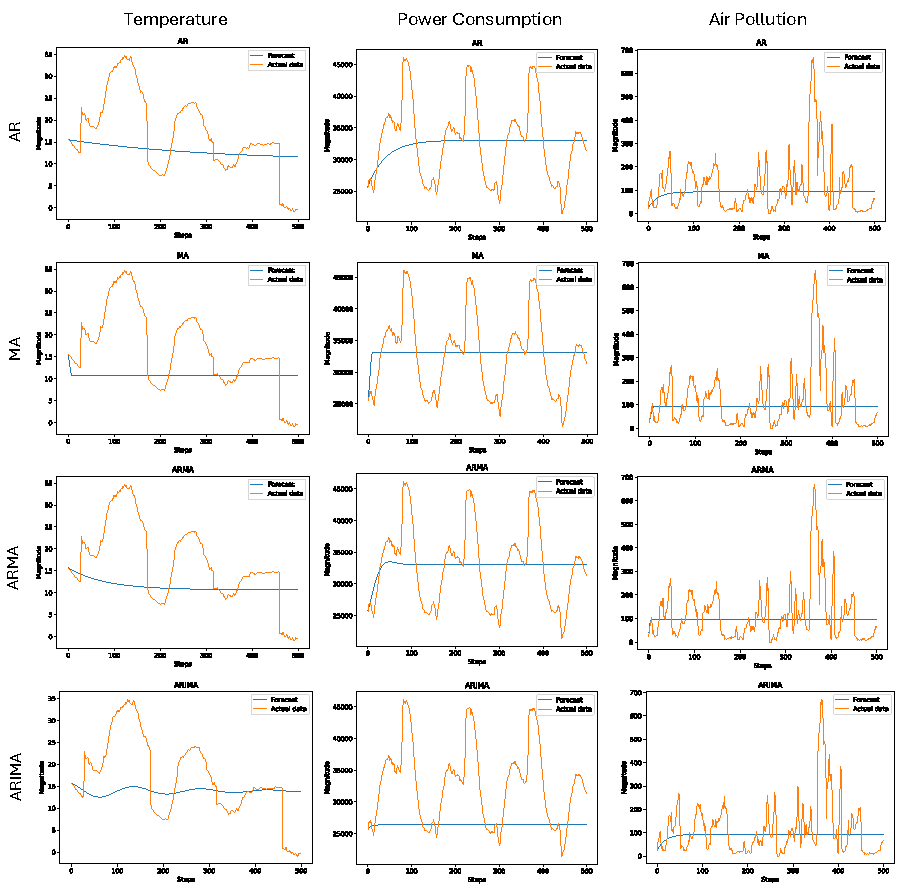
\includegraphics[scale=0.9]{Latex_report/fig/classical.pdf}
	\end{center}
	\caption{Classical Models: Prediction vs. Ground Truth}
	\label{fig:classical}
\end{figure}


\subsection{Modern techniques}
We implemented three modern techniques, including Long Short-Term Memory (LSTM), Bidirectional LSTM (BiLSTM), and Sequence-to-Sequence (Seq2Seq).


LSTM, a type of recurrent neural network (RNN), is designed to capture long-term dependencies in sequential data by utilizing specialized memory cells that allow the model to retain important information over long periods. BiLSTM, an extension of LSTM, processes data in both forward and backward directions, which enhances the model’s ability to understand context from both past and future time steps. The Seq2Seq model is a more complex architecture that employs two LSTM networks: an encoder to process the input sequence and a decoder to generate the output sequence. This model is particularly useful for tasks like sequence translation and time series forecasting, where there is a need to map input sequences to output sequences.

The three modern techniques were trained with identical hyperparameters, as outlined in Table \ref{tab:hyperparams}, as well as the same number of layers and hidden sizes. This setup ensures that the results are directly comparable across models, allowing us to isolate and assess the specific impact of each model’s architecture on performance.  MSE, RMSE, and MAE are also calculated to assess the performance, as summarized in Table \ref{tab:lstm_metric}. Figure \ref{fig: modern} illustrates the comparison between the predicted and actual values for LSTM, BiLSTM, and Seq2Seq models. The modern techniques demonstrate significantly better performance than the classical models, as reflected in their lower MSE values. Additionally, the comparison plots between predictions and actual values further highlight their superior accuracy. Among the three modern techniques, the LSTM model, despite having the simplest architecture, achieves the lowest MSE. This suggests that for the datasets used in this study, the straightforward architecture of the LSTM is sufficient to handle the tasks effectively.

\begin{table}[h!]
\centering
\begin{tabular}{@{}lccc@{}}
\toprule
\textbf{}               & \textbf{MSE} & \textbf{RMSE} & \textbf{MAE} \\ \midrule
\textbf{LSTM}           &              &               &              \\
Temperature             & 0.000127     & 0.011277      & 0.004017     \\
Power consumption       & 0.000175     & 0.013225      & 0.008923     \\
Air pollution           & 0.001260     & 0.035502      & 0.018459     \\ \midrule
\textbf{Bi-LSTM}        &              &               &              \\
Temperature             & 0.000131     & 0.011437      & 0.004310     \\
Power consumption       & 0.000179     & 0.013362      & 0.009071     \\
Air pollution           & 0.000261     & 0.035516      & 0.019128     \\ \midrule
\textbf{Seq2Seq}        &              &               &              \\
Temperature             & 0.000128     & 0.011307      & 0.004099     \\
Power consumption       & 0.000226     & 0.015046      & 0.009872     \\
Air pollution           & 0.000247     & 0.035312      & 0.018662       \\ \bottomrule
\end{tabular}
\caption{Metrics comparison for Modern Techniques. Both prediction and ground truth are normalized using the equation in \ref{nomalize}.}
\label{tab:lstm_metric}
\end{table}



\begin{figure}[H]
	\begin{center}
		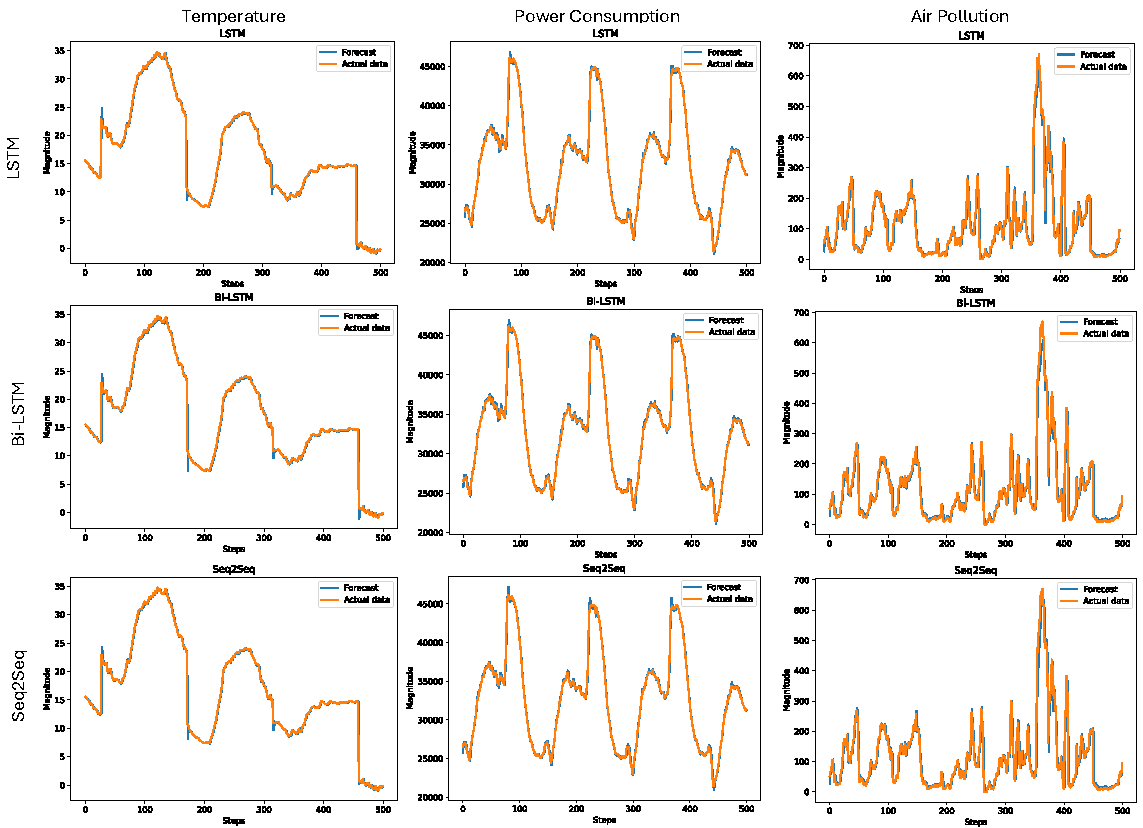
\includegraphics[scale=0.8]{Latex_report/fig/modern.pdf}
	\end{center}
	\caption{Modern Techniques: Prediction vs. Ground Truth}
	\label{fig:modern}
\end{figure}



\subsection{State of Art}
Finally, we utilized the Transformer model, which has recently become a state-of-the-art architecture due to its self-attention mechanism. The Transformer model allows for more parallelization and better capture of long-range dependencies compared to traditional RNN-based models. The self-attention mechanism enables the model to weigh the importance of different time steps when making predictions, significantly improving forecasting accuracy, especially in complex datasets. 
To ensure consistency in comparison, we used the same hyperparameters listed in Table \ref{tab:hyperparams} as those applied to modern techniques. Based on the prediction vs. actual plots in Figure \ref{fig: trans} and the metrics presented in Table \ref{tab:trans_metric}, the Transformer model outperforms the classical models we implemented. However, its performance does not surpass that of the three modern techniques. This suggests that for these three datasets, a complex Transformer architecture may not be necessary to achieve effective performance.



\begin{table}[h!]
\centering
\begin{tabular}{@{}lccc@{}}
\toprule
\textbf{}               & \textbf{MSE} & \textbf{RMSE} & \textbf{MAE} \\ \midrule
% \textbf{Transformer}    &              &               &              \\
Temperature             & 0.000599     & 0.024466      & 0.016530     \\
Power consumption       & 0.000467     & 0.021602      & 0.015685     \\
Air pollution           & 0.001370     & 0.037011      & 0.019526     \\ \bottomrule
\end{tabular}
\caption{Performance metrics for Transformer model. Both prediction and ground truth are normalized using the equation in \ref{nomalize}.}
\label{tab:trans_metric}
\end{table}


\begin{figure}[H]
	\begin{center}
		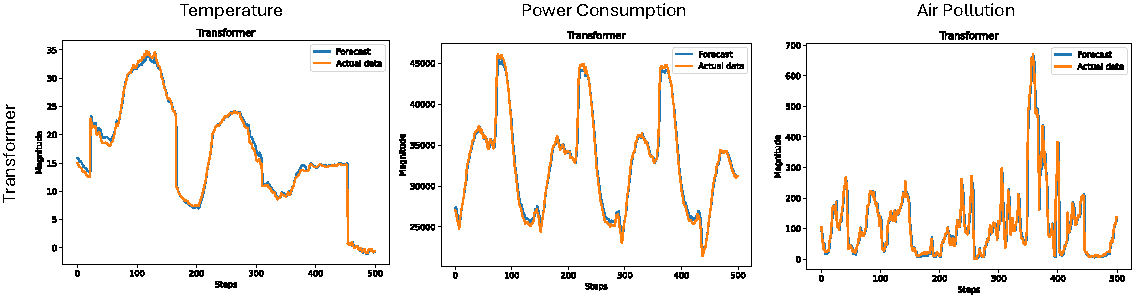
\includegraphics[scale=0.8]{Latex_report/fig/trans.pdf}
	\end{center}
	\caption{Transformer: Prediction vs. Ground Truth}
	\caption{Transformer: }
	\label{fig:trans}
\end{figure}




\subsection{Conclusion}
In this study, we evaluated the performance of four classical models (AR, MA, ARMA, ARIMA), three modern techniques (LSTM, BiLSTM, Seq2Seq), and a state-of-the-art Transformer model on three publicly available datasets. Overall, our findings indicate that while we implemented relatively simple classical models, both modern techniques and the Transformer model consistently outperformed the classical approaches. Among the deep learning-based models, LSTM, with its simplest architecture, achieved the lowest MSE. This suggests that even the simplest deep learning architecture is sufficient to handle the data effectively for these datasets.

However, there are some limitations to this study. For classical models, we selected relatively simple configurations based on available information, which may not represent their optimal performance. It is possible to identify better-performing classical models with more extensive exploration. Similarly, when using Optuna for hyperparameter tuning, we constrained the maximum potential order and the number of trials. Increasing these limits could lead to the discovery of more suitable models.

For modern techniques and the state-of-the-art Transformer model, we trained all models using a fixed sequence length and a common set of hyperparameters. However, these hyperparameters may not be the most optimal for each model or dataset.

Future work could include implementing Seasonal Autoregressive Integrated Moving Average (SARIMA) \cite{box2015time} models to better capture the strong seasonality present in the datasets. Additionally, employing advanced techniques like the Box-Jenkins \cite{box2015time} methodology and other model variations could provide a more comprehensive performance comparison. By addressing these limitations and exploring alternative approaches, we aim to further refine our findings and expand the scope of this research.


\bibliographystyle{IEEEtran}
\bibliography{references}


% %------ To create Appendix with additional stuff -------%
% %\newpage
% %\appendix
% %\section{Appendix}
% %Put data files, CAD drawings, additional sketches, etc.



\end{document} 